\section{Entorno de desarrollo de la solución}

Para llevar a cabo el desarrollo completo de la solución se debe recurrir a una 
gran cantidad herramientas, \textit{frameworks}, y recursos. En esta sección se 
describen estas tecnologías.

%En esta sección se describen todos las partes involucradas en el desarrollo de
%la solución propuesta. 

%La solución se compone de dos partes, la primera es la aplicación que los
%usuarios utilizan para realizar las prácticas, denominada \textit{Frontend}, y la segunda
%parte, es un servidor que se encarga de almacenar la información sobre los
%usuarios de la solución y como la utilizan, denominado \textit{Backend}.

%Primeramente se definen las herramientas de gestión de código, pues ellas son
%utilizadas tanto por la solución como por el \textit{backend}, luego se definen
%las herramientas específicas de la creación de la simulación y por último, se
%citan y describen de manera breve las herramientas utilizadas por el
%\textit{backend}.

%La idea detrás de separar la solución en \textit{Frontend} y \textit{Backend} 
%es que ambas partes de la solución se podrán mantener de forma separada sin que 
%el cambio de una afecte el funcionamiento de la otra. 

\subsection{Herramientas de gestión de código}

La gestión del código fuente desarrollado como parte de este trabajo de grado fue realizado
mediante la utilización de la herramienta de control de código fuente
\textit{Git}, \textit{Git} es un software de control de versiones distribuido,
de código abierto bajo la licencia \Gls{gnu}\cite{git}. El proveedor del
servicio \textit{Git} utilizado es \textit{BitBucket}\cite{bitbucket}, el cual
almacena repositorios \textit{Git}, la principal característica y motivación por
la cual se utiliza este servicio es que el mismo permite mantener varios
repositorios privados de manera gratuita\cite{bitbucket}.

\subsection{Desarrollo del \textit{front-end}}

El desarrollo de la solución requiere de una variedad importante de tecnologías
además del motor de videojuego, las herramientas descritas en esta sección complementan al
motor seleccionado y facilitan la creación de contenido.

En primer lugar, se utilizó el \Gls{ide} \textit{Unity Editor} para la creación de las escenas,
el \Gls{ide} \textit{MonoDevelop} y el lenguaje \cs{} para la programación de la
interacción entre los componentes de la solución.

Adicionalmente se utilizaron varias herramientas de diseño para crear
componentes 3D y 2D, \textit{Make Human} es utilizado para la creación de los
pacientes, \textit{3ds Max} permite la creación de objetos como gazas, y otros
elementos utilizados dentro de la solución. En cuanto a los gráficos 2D, se
utilizaron \textit{Photoshop}, y diversas páginas web que proveían contenido
gratuito.

\begin{itemize}

\item \textbf{Unity Editor}

El \Gls{ide} de \textit{Unity} es la herramienta en la se crean los videojuegos
o simulaciones. Este \Gls{ide} importa todos los \textit{asset}\footnote{Un
    \textit{Asset} es un paquete \textit{Unity} que puede contener modelos,
    librerias, sonidos, etc.}. Permite compilar las escenas con los terrenos,
luces, audios, personajes, física, entre otros. Se puede agregar interacción a
través de \textit{scripting}. Además se puede probar y editar en
forma simultánea los videojuegos y desplegarlos en las plataformas
elegidas\cite{unity3d}. 

Este editor es la única herramienta que permite crear escenas en \textit{Unity},
sin embargo, este \Gls{ide}, no permite la edición de código,\footnote{Existen
    \textit{Assets} que permiten la edición de código dentro del \textit{Unity
        Editor}, pero son pagas y de baja reputación} por ello se necesita un
editor externo de código.


\item \textbf{MonoDevelop}

\textit{MonoDevelop} es un \Gls{ide} de código abierto, bajo la licencia
\Gls{gnu} apoyado principalmente por la comunidad \textit{Mono}. Es el \Gls{ide}
utilizado por defecto en el desarrollo de aplicaciones para \textit{Unity3D}, el
mismo soporta varios lenguajes de programación, como \cs{},
\textit{UnityScript}, y \textit{Boo}. Es un \Gls{ide} multiplataforma que
soporta \textit{Windows} al igual que \textit{Unity3D}.

Existen otros editores que pueden ser utilizados para el desarrollo del código
fuente, pero los mismos no cuentan con el mismo nivel de integración y no son
gratuítos.\footnote{\textit{Microsoft Visual Studio} permite el mismo nivel de
    integración que \textit{MonoDevelop} con un \textit{plugin}, pero el mismo
    es de pago durante el desarrollo de la solución}

\item \textbf{\cs{}}

\textit{Unity3D} utiliza versiones limitadas\footnote{La definición del lenguaje
    es la misma, pero las librerías estándar no están completas}de tres
lenguajes de programación: \cs{}, \textit{UnityScript}, y
\textit{Boo}\cite{unity:script}. Estos lenguajes son compilados y orientados a
objetos.

Otra característica interesante es que, por el orden de compilación de los
proyectos \textit{Unity3D}, los archivos \textit{UnityScript} y \textit{Boo} son
compilados antes que los archivos \cs{}, esto provoca que, las clases
\textit{UnityScript} sean utilizables desde \cs{}, lo que no se cumple en el
caso contrario, es decir, las clases \cs{} no son accesibles desde código
\textit{UnityScript} o \textit{Boo}.

Por lo mencionado anteriormente se selecciona a \cs{} como el lenguaje de
implementación. Además, es el lenguaje con más ayuda en línea, y las
librerías no diseñadas específicamente para \textit{Unity3d} pueden ser
utilizadas. Otro factor que influye en la elección es la familiaridad de los
autores con lenguajes similares. 

\item \textbf{Herramientas de diseño}

Las herramientas utilizadas para crear modelos 3D e imágenes 2D son las siguientes:

\begin{itemize}
\item \textbf{MakeHuman}: es un software de código abierto bajo la licencia
    \Gls{agnu} para crear personajes humanos 3D. Es una herramienta diseñada
    para simplificar la creación de seres humanos virtuales utilizando una
    interfaz gráfica de usuario\cite{makehuman}. 
\item \textbf{3ds Max}: es un software privado de modelado 3D, que además posee
    herramientas para animación, simulación y renderización. Esta herramienta
    fue utilizada para crear objetos 3D que no fueran personajes humanos y para
    exportar modelos de un formato a otro que fuera compatible con
    \textit{Unity3D}\cite{3dsmax}.
\item \textbf{Photoshop}: es una herramienta de edición de gráficos 2D de
    \textit{Adobe}, permite la creación y edición de gráficos, es utilizada para
    la creación de iconos, botones y otro contenido 2D que forma parte de la
    solución.
\end{itemize}

\end{itemize}


\subsection{Desarrollo del \textit{back-end}}

Para registrar las actividades del usuario en el front-end, se necesita de un
servidor que almacene los datos de todos los usuarios y las actividades que
estos realizan dentro de la solución.

En la figura~\ref{fig:backend_diagrama} se puede observar en lineas generales
como funciona este servicio, desde el registro de actividades del usuario, la
comunicación con el \textit{back-end}, su posterior traducción y persistencia en
una base datos, así, este servicio debe proveer:

\begin{itemize}
    \item \textbf{Alta disponibilidad}: el servidor debe estar disponible en
        todo momento, cualquier día de la semana y a cualquier hora. Los
        requisitos de accesibilidad son estrictos, pues se necesita que los
        usuarios envíen datos sin inconvenientes cuando crean necesario.
    \item \textbf{Accesibilidad}: el servidor debe poder ser accesible desde
        cualquier red móvil.
    \item \textbf{Bajo costo de comunicación}: la comunicación del usuario con
        el \textit{back-end} debe ser lo menos costosa posible, pues se utilizan
        recursos del usuario.
\end{itemize}

\begin{figure}[H]
\centering
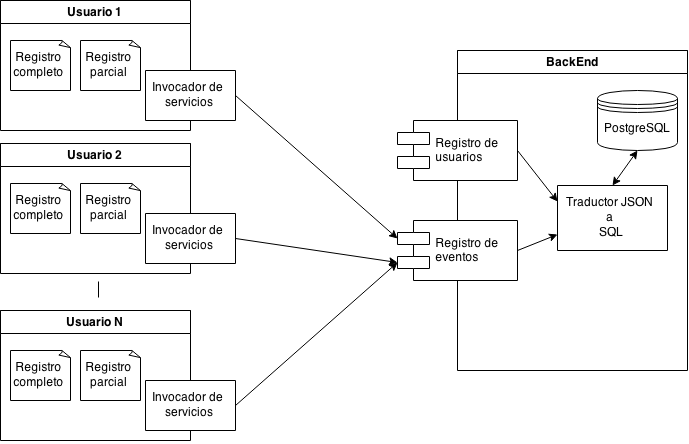
\includegraphics[scale=0.4]{tecnologias/images/backend_diagrama.png}
\caption{Diagrama de la interacción de los usuarios con el \textit{back-end}, se
    puede observar a grandes rasgos, los componentes del sistema y los servicios
    que ofrece.}
\label{fig:backend_diagrama}
\end{figure}

Las tecnologías utilizadas para el desarrollo del \textit{back-end} son:

\begin{itemize}
\item \textbf{\Gls{javaee}}

Para el desarrollo de la aplicación web que almacena los datos se utiliza
\Gls{javaee} en su versión $6$, la misma se utiliza por la familiarización de
los autores con la tecnología y la facilidad que provee para la
realización de servicios web que permitan la interacción con la solución.

\item \textbf{\Gls{rest}}

Para los servicios se utiliza la arquitectura \Gls{rest}, la principal
motivación para utilizar \Gls{rest} es la eficiencia en el uso de la
red\cite{pautasso2008restful}, la cual es también la motivación para la
utilización de \Gls{json}. La implementación del lado del servidor de la
arquitectura \Gls{rest} es \textit{RestEasy}, de parte del \textit{front-end} se utiliza
la implementación por defecto de \textit{Unity3D}.

\item \textbf{PostgresSQL}

El almacenamiento permanente de los datos se logra con la utilización de
\textit{PostgreSQL}, el cual es un motor de bases de datos de código abierto
dirigido por \textit{PostgreSQL Global
    Development Group}. La versión elegida es la $9.1$.

\item \textbf{OpenShift}

A fin de obtener las características necesarias, de alta disponibilidad y
accesibilidad, se utiliza la herramienta de plataforma como servicio de
\textit{RedHat} llamada \textit{OpenShift}, la cual es un producto de código
abierto dirigido por \textit{RedHat}.

Además de dirigir el proyecto, \textit{RedHat} provee un servicio limitado y
gratuito\cite{openshift:pricing}.\footnote{Existen versiones completas del
    producto mantenidas por \textit{RedHat}, las cuales tienen un costo mensual
    y de acuerdo a las funcionalidades utilizadas\cite{openshift:pricing}} Para
esta tesis se utilizo el servicio gratuito con la plataforma \textit{JBoss
    Application Server 7.1} y \textit{PostgreSQL 9.1}.

\end{itemize}

\section{Resumen}

A modo de resumen de las tecnologías utilizadas para el desarrollo de la solución
propuesta se presentan las tablas~\ref{tab:stack_tecnologico_fe} y~\ref{tab:stack_tecnologico_be}.

\begin{table}[H]
\centering
\begin{tabular}{lrr}
\toprule
\textbf{Utilización} & \textbf{Tecnología} & \textbf{Versión} \\
\midrule
Motor de videojuego      & Unity3d         & 4.5 \\
IDE                      & MonoDevelop     & 4 \\
                         & Unity Editor    & 4.5 \\
\midrule
Modelado 3D              & 3ds Max         & 2013 \\
Modelado 2D              & Photoshop       & 14 \\
Modelado de personajes   & MakeHuman       & 1.0 \\

\midrule
Lenguaje de programación & \cs{} \\
Gestión de código fuente & GIT & 1.8 \\
Otras librerías          & NGUI            & 2.7\\
                         & Facebook \\
                         
\bottomrule
\end{tabular}
\caption{Resumen de las tecnologías utilizadas en el \textit{front-end}}
\label{tab:stack_tecnologico_fe}
\end{table}


\begin{table}[H]
\centering
\begin{tabular}{lrr}
\toprule
\textbf{Utilización} & \textbf{Tecnología}  & \textbf{Versión} \\
\midrule
IDE                         & Eclipse & Luna\\
Lenguaje de programación    & Java & 7\\
\midrule
Servidor de aplicaciones    & Jboss & 7 \\
Servidor de base de datos   & PostgreSQL & 9.2 \\
Proveedor de plataforma     & OpenShift \\
\midrule
Gestión de código fuente    & GIT & 1.8\\
Otras librerias             & Java EE & 6\\

\bottomrule
\end{tabular}
\caption{Resumen de las tecnologías utilizadas en el \textit{back-end}}
\label{tab:stack_tecnologico_be}
\end{table}
